% Slides for 2024-07-23
% To create a slide, use the following:
\begin{frame}{Accuracy with different epochs and learning rates}
    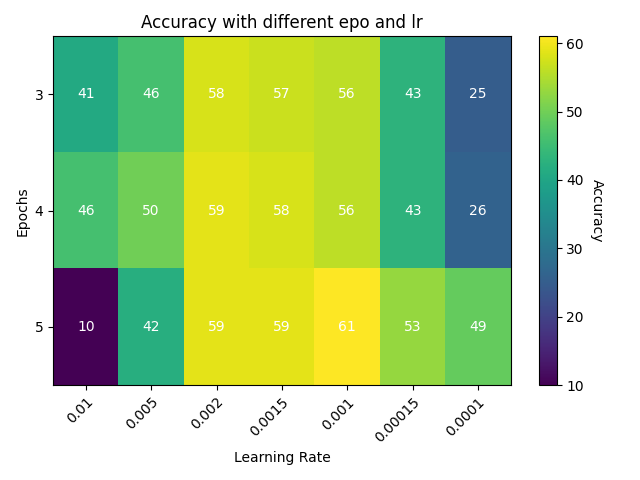
\includegraphics[scale=.6]{images/accuracy with different epo and lr.png}
\end{frame}

\begin{frame}{Loss with different widths}
    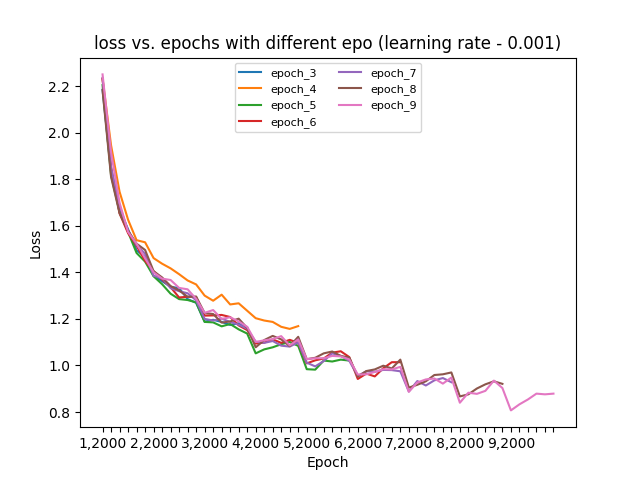
\includegraphics[scale=.6]{images/loss vs. epochs with different epo (learning rate - 0.001).png}
\end{frame}

\begin{frame}{Loss with different learning rates and epochs}
    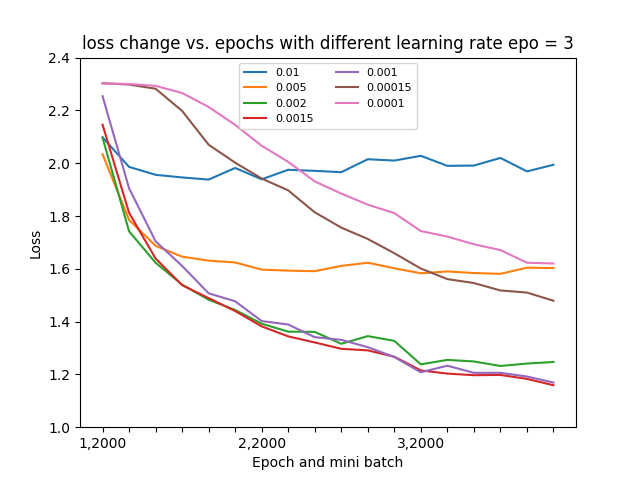
\includegraphics[scale=.3]{images/loss change vs. epochs with different learning rate epo = 3.png}
    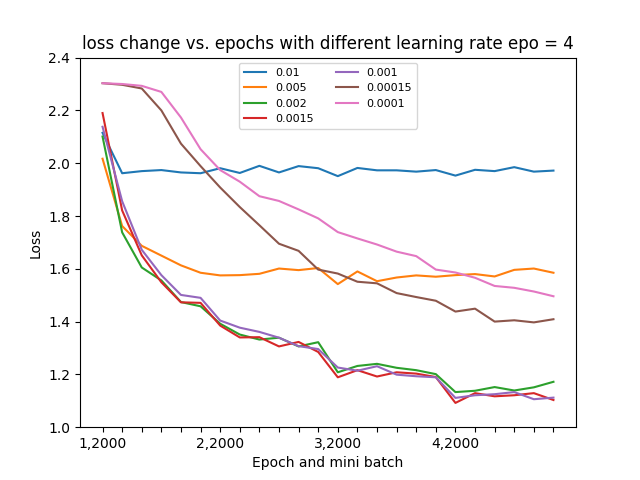
\includegraphics[scale=.3]{images/loss change vs. epochs with different learning rate epo = 4.png}
    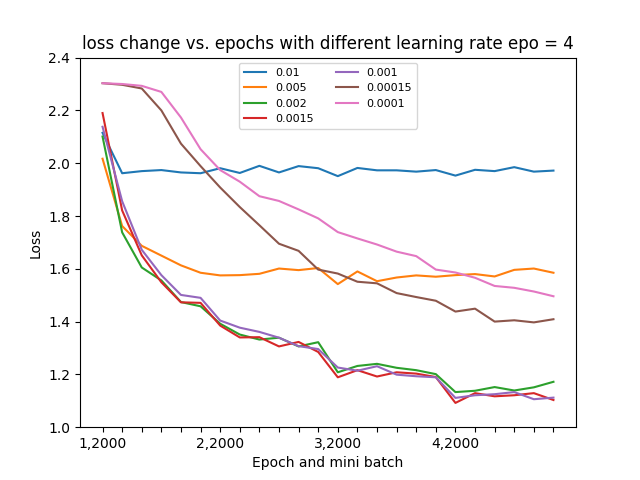
\includegraphics[scale=.3]{images/loss change vs. epochs with different learning rate epo = 4.png}
\end{frame}

\begin{frame}{Loss with different widths}
    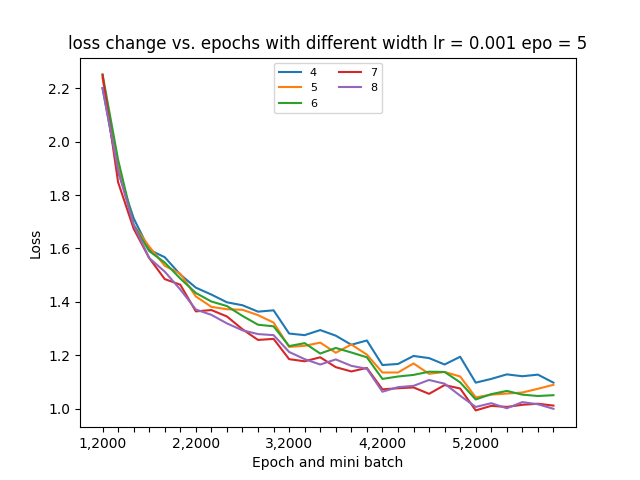
\includegraphics[scale=.6]{images/loss change vs. epochs with different width lr 0.001 epo 5.png}
\end{frame}

\begin{frame}{work this week}
    refactor the code
\end{frame}
% To create a slide with a bullet list, use the following:
% \begin{frame}{TITLE}
%     \begin{itemize}
%         \item ITEM 1
%         \item ITEM 2
%     \end{itemize}    
% \end{frame}

% To create a slide with numbered list, use the following:
% \begin{frame}{TITLE}
%     \begin{enumerate}
%         \item ITEM 1
%         \item ITEM 2
%     \end{enumerate}
% \end{frame}

% To create a slide with a graphic:
% 1. Add the graphic to this folder (named picture.png)
% 2. Use the following:
% \begin{frame}{TITLE}
%     \centering
%     \includegraphics[height=0.7\textheight,width=0.7\textwidth,keepaspectratio]{picture.png}
% \end{frame}

% To create a slide with two columns, use the following:
% \begin{frame}{TITLE}
%     \begin{columns}
%         \begin{column}{0.5\textwidth}
%             COLUMN 1 BODY
%         \end{column}
%         \begin{column}{0.5\textwidth}
%             COLUMN 2 BODY
%         \end{column}
%     \end{columns}
% \end{frame}
